% PGF/TikZ picture from SSJ 
% XScale = 10.0,  YScale = 10.0,  XShift = -6.0,  YShift = -4.0
% Therefore, thisFileXValue = (originalSeriesXValue+XShift)*XScale
%        and thisFileYValue = (originalSeriesYValue+YShift)*YScale

\begin{center}
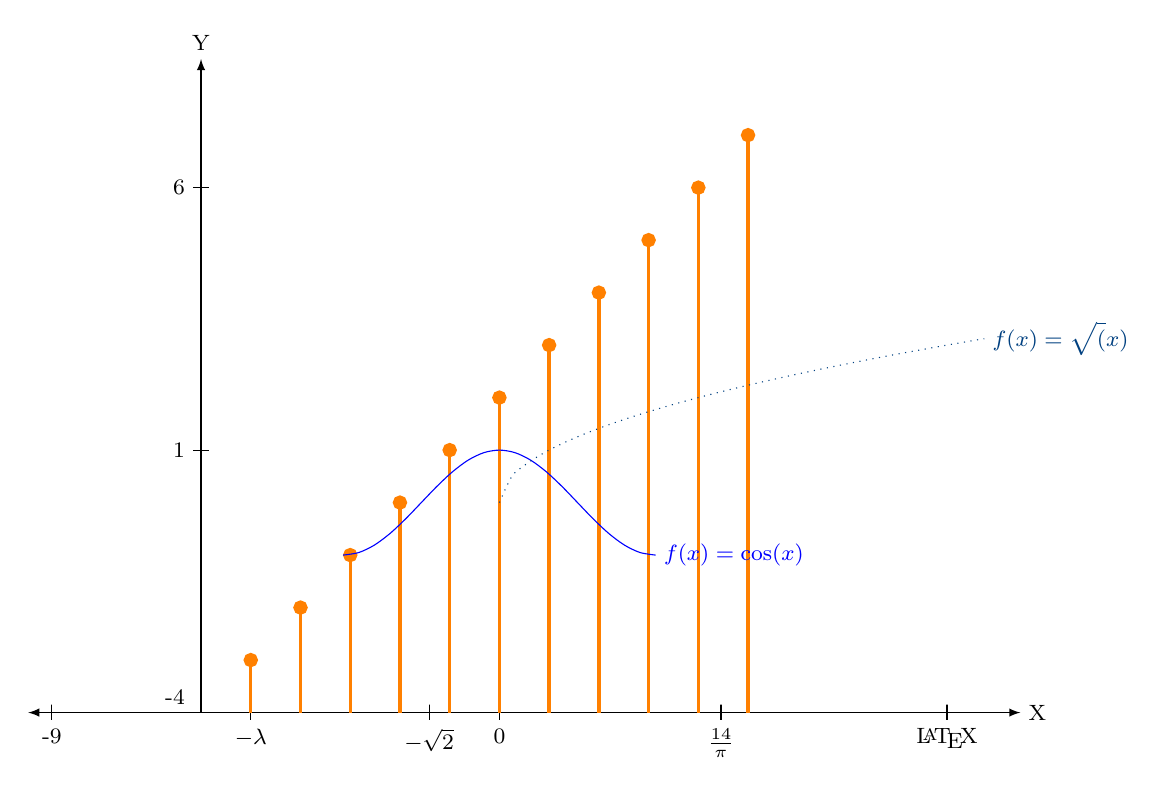
\begin{tikzpicture}[x=0.06315789473684211cm, y=0.06666666666666667cm]
\footnotesize
\draw [latex-latex] ([xshift=-3mm] -30.0,0) -- ([xshift=3mm] 160.0,0) node[right] {X};
\draw (-30.0,0) -- +(0mm,1mm) -- +(0mm,-1mm) node[below] {-9};
\draw (10.0,0) -- +(0mm,1mm) -- +(0mm,-1mm) node[below] {$-\lambda$};
\draw (45.85786437626905,0) -- +(0mm,1mm) -- +(0mm,-1mm) node[below] {$-\sqrt{2}$};
\draw (60.0,0) -- +(0mm,1mm) -- +(0mm,-1mm) node[below] {0};
\draw (104.5633840657307,0) -- +(0mm,1mm) -- +(0mm,-1mm) node[below] {$\frac{14}{\pi}$};
\draw (150.0,0) -- +(0mm,1mm) -- +(0mm,-1mm) node[below] {\LaTeX};
\draw [-latex] ([yshift=-0mm] 0,0.0) -- ([yshift=3mm] 0, 120.0) node[above] {Y};
\draw (0,0.0) -- +(1mm,0mm) -- +(-1mm,0mm) node[above left] {-4};
\draw (0,50.0) -- +(1mm,0mm) -- +(-1mm,0mm) node[left] {1};
\draw (0,100.0) -- +(1mm,0mm) -- +(-1mm,0mm) node[left] {6};
\draw [ycomb,very thick, color=orange, mark=*, style=solid] plot coordinates {%
(10.00,10.0000) %   (-5.000000,  -3.000000)
(20.00,20.0000) %   (-4.000000,  -2.000000)
(30.00,30.0000) %   (-3.000000,  -1.000000)
(40.00,40.0000) %   (-2.000000,  0.000000)
(50.00,50.0000) %   (-1.000000,  1.000000)
(60.00,60.0000) %   (0.000000,  2.000000)
(70.00,70.0000) %   (1.000000,  3.000000)
(80.00,80.0000) %   (2.000000,  4.000000)
(90.00,90.0000) %   (3.000000,  5.000000)
(100.00,100.0000) %   (4.000000,  6.000000)
(110.00,110.0000)} %   (5.000000,  7.000000)
 node[right] { };
\draw [smooth, color=blue, mark=, style=solid] plot coordinates {%
(28.58,30.0000) %   (-3.141593,  -1.000000)
(31.73,30.4894) %   (-2.827433,  -0.951057)
(34.87,31.9098) %   (-2.513274,  -0.809017)
(38.01,34.1221) %   (-2.199115,  -0.587785)
(41.15,36.9098) %   (-1.884956,  -0.309017)
(44.29,40.0000) %   (-1.570796,  0.000000)
(47.43,43.0902) %   (-1.256637,  0.309017)
(50.58,45.8779) %   (-0.942478,  0.587785)
(53.72,48.0902) %   (-0.628319,  0.809017)
(56.86,49.5106) %   (-0.314159,  0.951057)
(60.00,50.0000) %   (0.000000,  1.000000)
(63.14,49.5106) %   (0.314159,  0.951057)
(66.28,48.0902) %   (0.628319,  0.809017)
(69.42,45.8779) %   (0.942478,  0.587785)
(72.57,43.0902) %   (1.256637,  0.309017)
(75.71,40.0000) %   (1.570796,  0.000000)
(78.85,36.9098) %   (1.884956,  -0.309017)
(81.99,34.1221) %   (2.199115,  -0.587785)
(85.13,31.9098) %   (2.513274,  -0.809017)
(88.27,30.4894) %   (2.827433,  -0.951057)
(91.42,30.0000)} %   (3.141593,  -1.000000)
 node[right] {$f(x) = \cos(x)$};
\definecolor{color0}{rgb}{0.00, 0.25, 0.50}
\draw [smooth, color=color0, mark=, style=dotted] plot coordinates {%
(60.00,40.0000) %   (0.000000,  0.000000)
(62.50,45.0000) %   (0.250000,  0.500000)
(65.00,47.0711) %   (0.500000,  0.707107)
(67.50,48.6603) %   (0.750000,  0.866025)
(70.00,50.0000) %   (1.000000,  1.000000)
(72.50,51.1803) %   (1.250000,  1.118034)
(75.00,52.2474) %   (1.500000,  1.224745)
(77.50,53.2288) %   (1.750000,  1.322876)
(80.00,54.1421) %   (2.000000,  1.414214)
(82.50,55.0000) %   (2.250000,  1.500000)
(85.00,55.8114) %   (2.500000,  1.581139)
(87.50,56.5831) %   (2.750000,  1.658312)
(90.00,57.3205) %   (3.000000,  1.732051)
(92.50,58.0278) %   (3.250000,  1.802776)
(95.00,58.7083) %   (3.500000,  1.870829)
(97.50,59.3649) %   (3.750000,  1.936492)
(100.00,60.0000) %   (4.000000,  2.000000)
(102.50,60.6155) %   (4.250000,  2.061553)
(105.00,61.2132) %   (4.500000,  2.121320)
(107.50,61.7945) %   (4.750000,  2.179449)
(110.00,62.3607) %   (5.000000,  2.236068)
(112.50,62.9129) %   (5.250000,  2.291288)
(115.00,63.4521) %   (5.500000,  2.345208)
(117.50,63.9792) %   (5.750000,  2.397916)
(120.00,64.4949) %   (6.000000,  2.449490)
(122.50,65.0000) %   (6.250000,  2.500000)
(125.00,65.4951) %   (6.500000,  2.549510)
(127.50,65.9808) %   (6.750000,  2.598076)
(130.00,66.4575) %   (7.000000,  2.645751)
(132.50,66.9258) %   (7.250000,  2.692582)
(135.00,67.3861) %   (7.500000,  2.738613)
(137.50,67.8388) %   (7.750000,  2.783882)
(140.00,68.2843) %   (8.000000,  2.828427)
(142.50,68.7228) %   (8.250000,  2.872281)
(145.00,69.1548) %   (8.500000,  2.915476)
(147.50,69.5804) %   (8.750000,  2.958040)
(150.00,70.0000) %   (9.000000,  3.000000)
(152.50,70.4138) %   (9.250000,  3.041381)
(155.00,70.8221) %   (9.500000,  3.082207)
(157.50,71.2250)} %   (9.750000,  3.122499)
 node[right] {$f(x) = \sqrt(x)$};
\end{tikzpicture}
\end{center}

